\chapter{Enriching impurities in hydrogen refuelling station samples}

\section*{Abstract}
In this chapter the HIED  was tested under a number of conditions using a commercial membrane compared against the best performing fabricated membranes in chapter 5. 

Enrichment was performed using a number of synthetic hydrogen samples created using the procedure outlined in section \ref{exp-gasprep}, and a hydrogen sample taken from a hydrogen refuelling station. The device was capable of enriching samples to 85 times. Theoretically higher enrichment factors were possible but these tests were limited for safety reasons. The commercial membrane took 7 days to perform this measurement and provided the final value of within 2\% of the gravametrically calculated value using the tracer enrichment method which was deemed sufficient for a commercial device. The device was also tested using a sulphur containing sample which resulted in failure of all membranes. The PdCuZr membrane while identified as being a strong candidate for enriching sulphurous impurities, failed in all tests due to poor thermal stability of the support. The commercial membrane on the other hand reacted with the gases in the mixture and became completely inactive. 

For the first time a sample was taken dierctly from a hydrogen refuelling station and enriched. The sample was enriched 46 times and was found to have 22 ppm of nitrogen, and a small amount of argon which was not visible during other tests, further showing that the method can be used to quantify impurities past the limit of detection normally achievable.   

\section{Introduction}
Now that appropriate membrane compositions have been found, a number of improvements must be made to the hydrogen impurity enrichment device in order to make it suitable as a commercial process and product for measuerment of ISO 14687-2 impurities. All previous devices used were extremely manual and required close operator attention to ensure the experiment performed correctly. All enrichment factor calculations discussed in section \ref{exp-enrichproc} must also be calculated by hand, after the experiment has been performed, limiting the ability for the operator to plan the experiment in advance. In addition to this the krypton enrichment method which was identified as the best method for calculating the enrichment factor in section \ref{lit-enrichlit} but no procedure is in place to instruct operators on how to add this krypton to their sampling vessel. 

This chapter will provide a method for taking krypton spiked samples from a hydrogen refuelling station, improve the hydrogen impurity enrichment device through automation to improve the usability of the device, while providing real time results for the user, and quantify how the enrichment device performs when tested using a real sample froma  hydrogenr refuelling station. 

\section{Enrichment of hydrogen samples}
Enrichment of the hydrogen samples was performed using the set up shown in figure \ref{hiedpid}. An initial test was performed using a commercial membrane supplied by REB using an inert mixture created using the procedure in section \ref{exp-gasprep} in order to calculate the uncertainty associated with the device. Both the commercial and PdCuZr membrane identified as the best performing membrane in chapter 5 were tested using a synthetic gas mixture containing sulphur containing compounds, and krypton. Finally both the commercial membrane and PdCuZr membrane were tested using a sample taken from the hydrogen refuelling station using the procedure outlined in section \ref{exp-sampletake}.

In each case the system was purged 7 times with the hydrogen sample to ensure there was no air present in the system. Enrichment was performed at a temperature of 300\textdegree C and a final enrichment pressure of 5 bar. Enrichment factors were calculated using both the tracer enrichment method (equation \ref{lit-eq:2}) calculated at the end of the test, and non-ideal gas law method (\ref{lit-eq:2}) calculated using the data processing script described in section \ref{dataproc}.

The gas mixtures used in the inert and sulphur tests are shown in table \ref{inert} and \ref{exp-sulf}. Prior to testing the HRS sample was tested to verify the concentration of krypton, and ensure there was no oxygen present in the system to pose as a hazard. Enrichment factors were capped at 100 to ensure any residual oxygen would not reach a high enough concentration to create an explosive environment.

\begin{table}[]
    \centering
    \caption{Gas mixture composition of the inert sample used during enrichment tests}
    \label{inert}
    \begin{tabular}{@{}cc@{}}
    \toprule
    Impurity & \begin{tabular}[c]{@{}c@{}}Concentration \\ ($\mu$mol/mol)\end{tabular} \\ \midrule
    N\textsubscript{2}       & 6.67 ± 0.06                                                               \\
    Kr       & 5.984 ± 0.06                                                               \\
    H\textsubscript{2}       & Balance                                                             \\ \bottomrule
    \end{tabular}
    \end{table}

\subsection{Inert components}\label{inertsec}
The inert mixture in table \ref{inert} was enriched to a CEF value of approximately 85. The enrichment period was performed over a 7 day period due to the low flux value achieved by the commercial membrane supplied. The $CEF_{NI}$ value was calculated using the algorithm decscibed in section \ref{dataproc} and can it's progress over the 7 day period shown in figure \ref{GCNI}. The $CEF_{NI}$ slightly overshot the desired value of 85, stabilising at a value of 84.33 ± 9.24, and as can be seen varied widely over the course of the experiment due to signal noise and interference. The value is still useful for keeping track of the progress of the experiment. 

The system was not operated continuously for 180 hours, and was switched off at night when monitoring was not possible. This is why the $CEF_{NI}$ value fluctuated over time. 

\begin{landscape}
    \begin{figure}
        \centering
        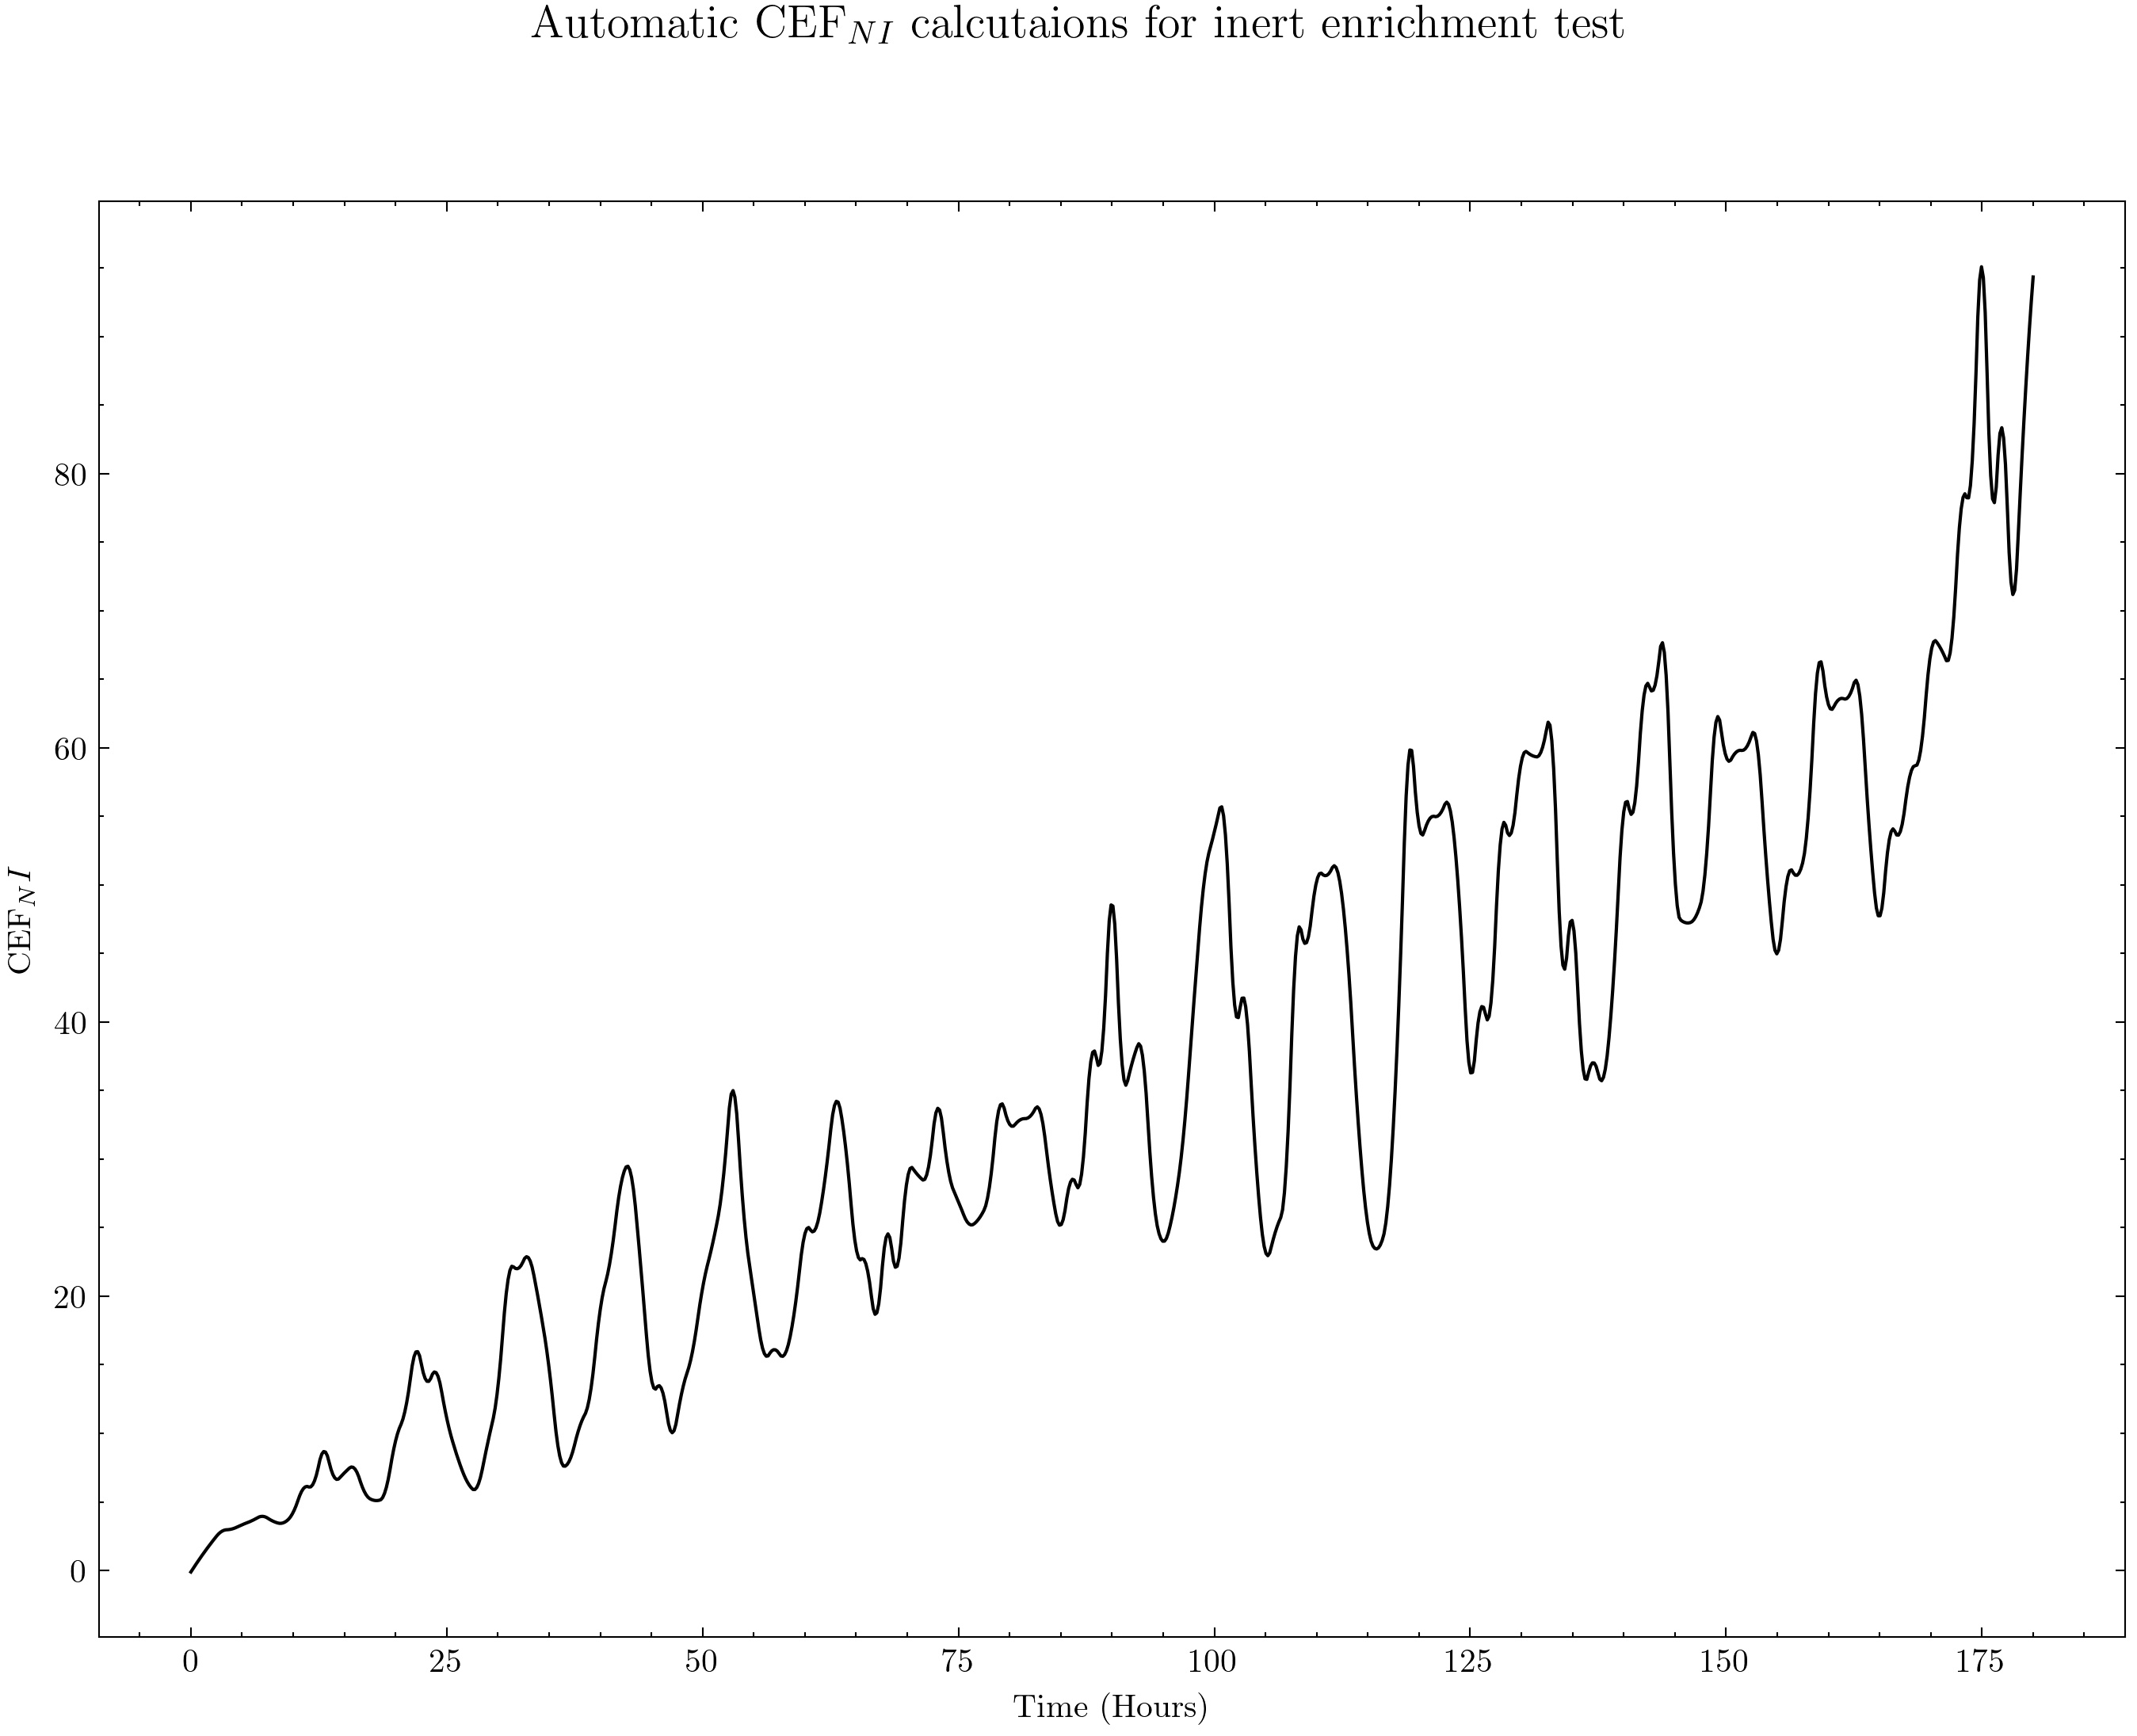
\includegraphics[width=0.9\linewidth, keepaspectratio]{/Users/marc/Thesis/Chapter5/inertenrich.jpg}
        \caption{$CEF_{NI}$ over the 180 hour enrichment of the inert hydrogen sample shown in table \ref{inert}}
        \label{GCNI}
    \end{figure}
\end{landscape}

Once the enrichment was complete, the system was isolated and left to cool. The transportable unit was then disconnected and it's composition measured and compared with it's original composition. Results were compared to nitrogen samples containing 251 nmol/mol, 500.77 nmol/mol, 1064 nmol/mol, 1437.37 nmol/mol using a derived calibration curve to account for non-linearity of the detector. The GC-PDHID data is shown in figure \ref{GCinert}. This analysis found that the enriched gas contained 514.62 ± 52 \textmu mol/mol of krypton and 570 ± 60 \textmu mol/mol of Nitrogen. Calculating the $CEF_T$ using the tracer enrichment method gave a value of 86 ± 9 . 

The calculation using $CEF_{NI}$ gave an initial Nitrogen concentration of 6.11 \textmu mol/mol (-7\%)N\textsubscript{2}. The tracer enrichment method calculated a value of 6.48 \textmu mol/mol (-1.7\%) further showing that the tracer enrichment method provides a more accurate result. 

\begin{figure}[H]
    \centering
    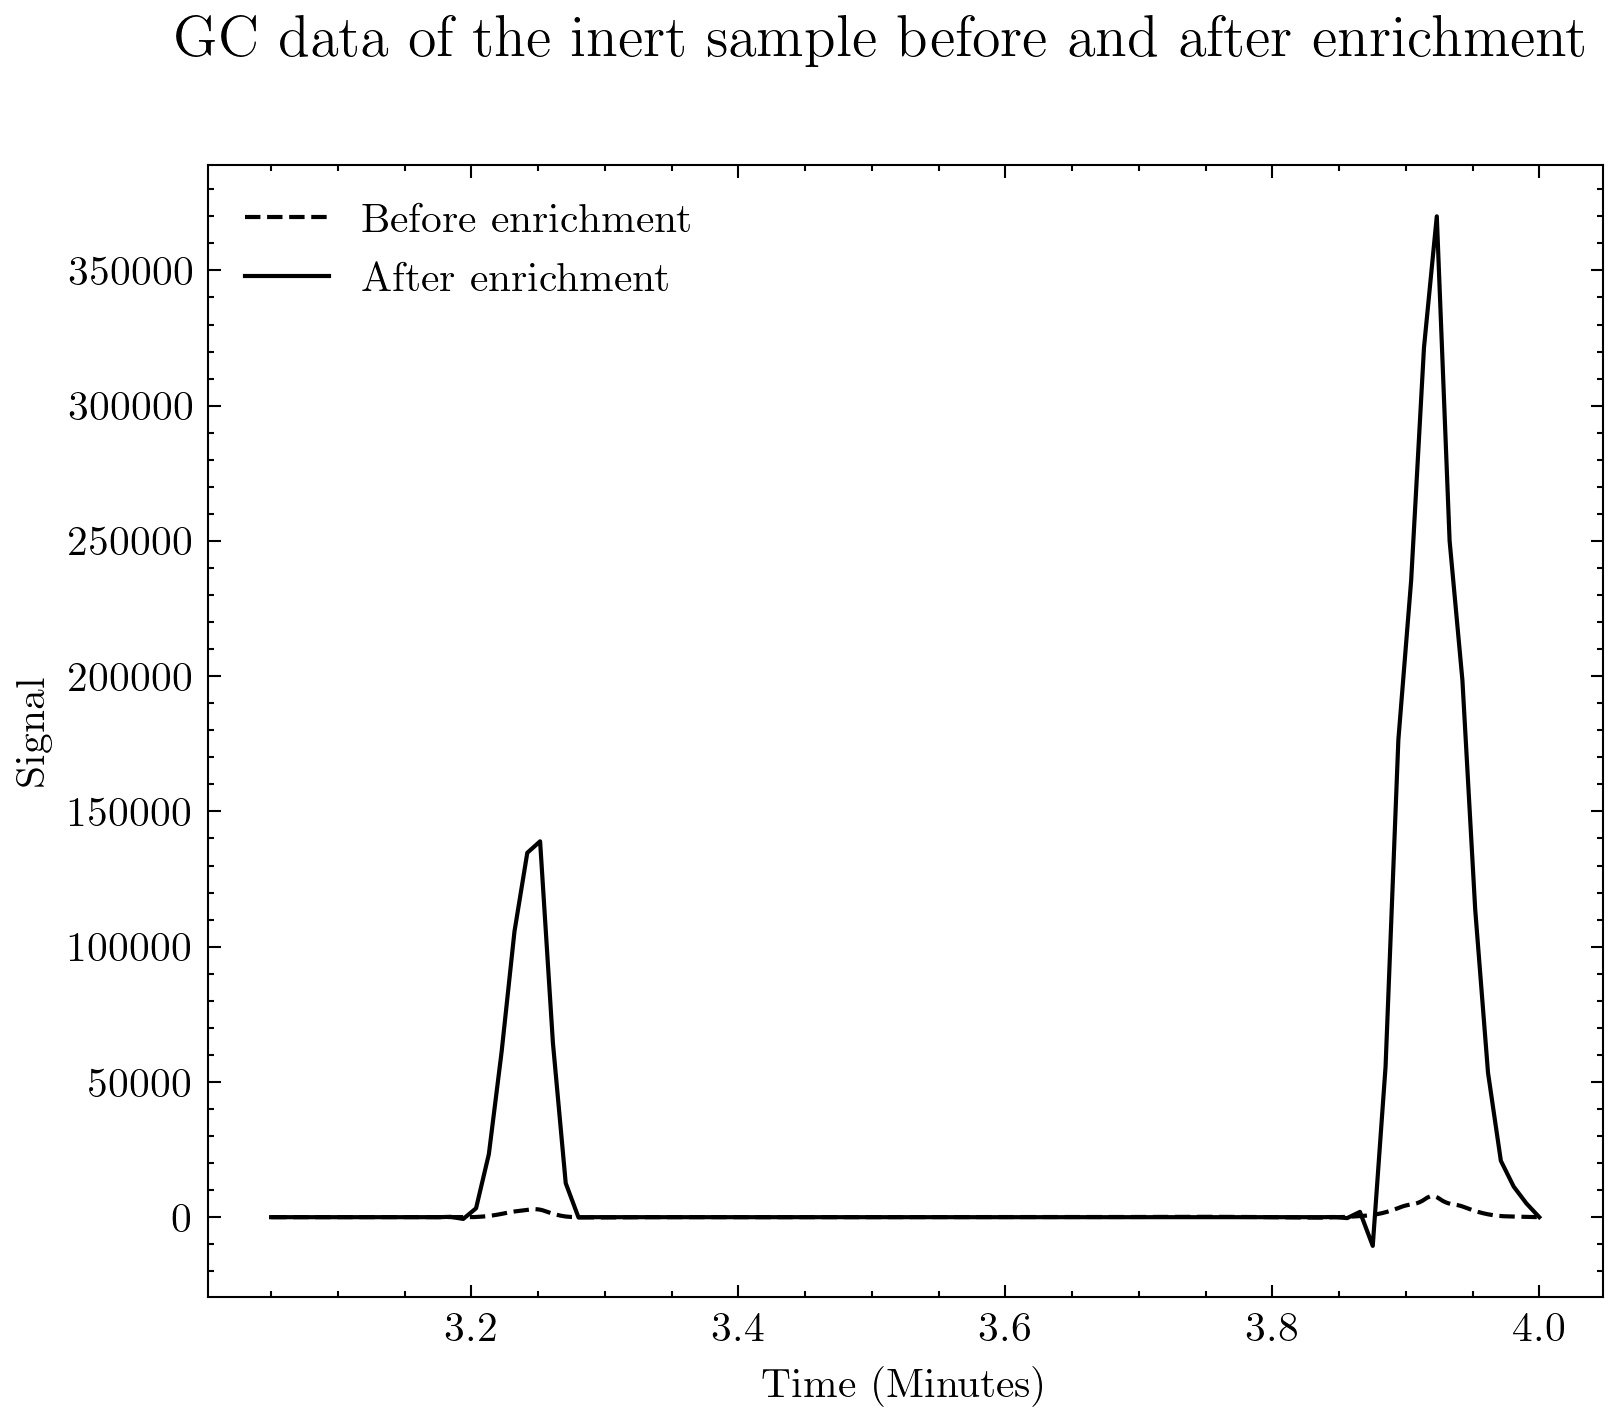
\includegraphics[width=\linewidth, keepaspectratio]{/Users/marc/Thesis/Chapter5/inertgc.jpg}
    \caption{GC-PDHID data of the inert sample both before and after enrichment with N\textsubscript{2} peaks shown at Time=3.25, and Kr peaks shown at Time=3.92}
    \label{GCinert}
\end{figure}

\subsection{Sulphur containing compounds}
The sulphur containing samples were tested using the same set up as section \ref{inertsec}, with the commercial PdAgAu membrane, and the PdCuZr alloy manufactured in chapter \label{proc-testingchapref}. The $CEF_{NI}$ values calculated in line for the experiment are shown in figure \ref{GCSULF}.

The commercial membrane saw the same dramatic drop in permeability as observed in chapter \ref{proc-testingchapref}. The experiment continued however it became clear that the permeability of the commercial membrane was dropping as the experiment went on, eventually becoming inactive to hydrogen permeability. The experiment was stopped. Upon analysis of the gas remaining within the enrichment vessel it was noted that the composition had significantly changed. This is shown in figure \ref{GCSULFCOMM}. The OCS, t-BuSH, THT and CS\textsubscript{2} in the gas mixture had reacted with the hydrogen to form H\textsubscript{2}S. While this would not effect the results of analysis much, sine the ISO 14687-2 standard does not give a maximum level of a specific sulphur containing compound, only the total concentration, OCS, THT, T-BuSH and CS\textsubscript{2} all contain carbon molecules. The result of this could be the formation of hydrocarbons, CO, or solid carbon on the surface of the membrane. In the case of carbon deposition, this would explain the complete deactivation of the membrane as discussed previously in section \ref{lit-pdreview}. In order to prevent this the exact reactions should be determined and process parameters further optimised to inhibit them from taking place. 

\begin{figure}[H]
    \centering
    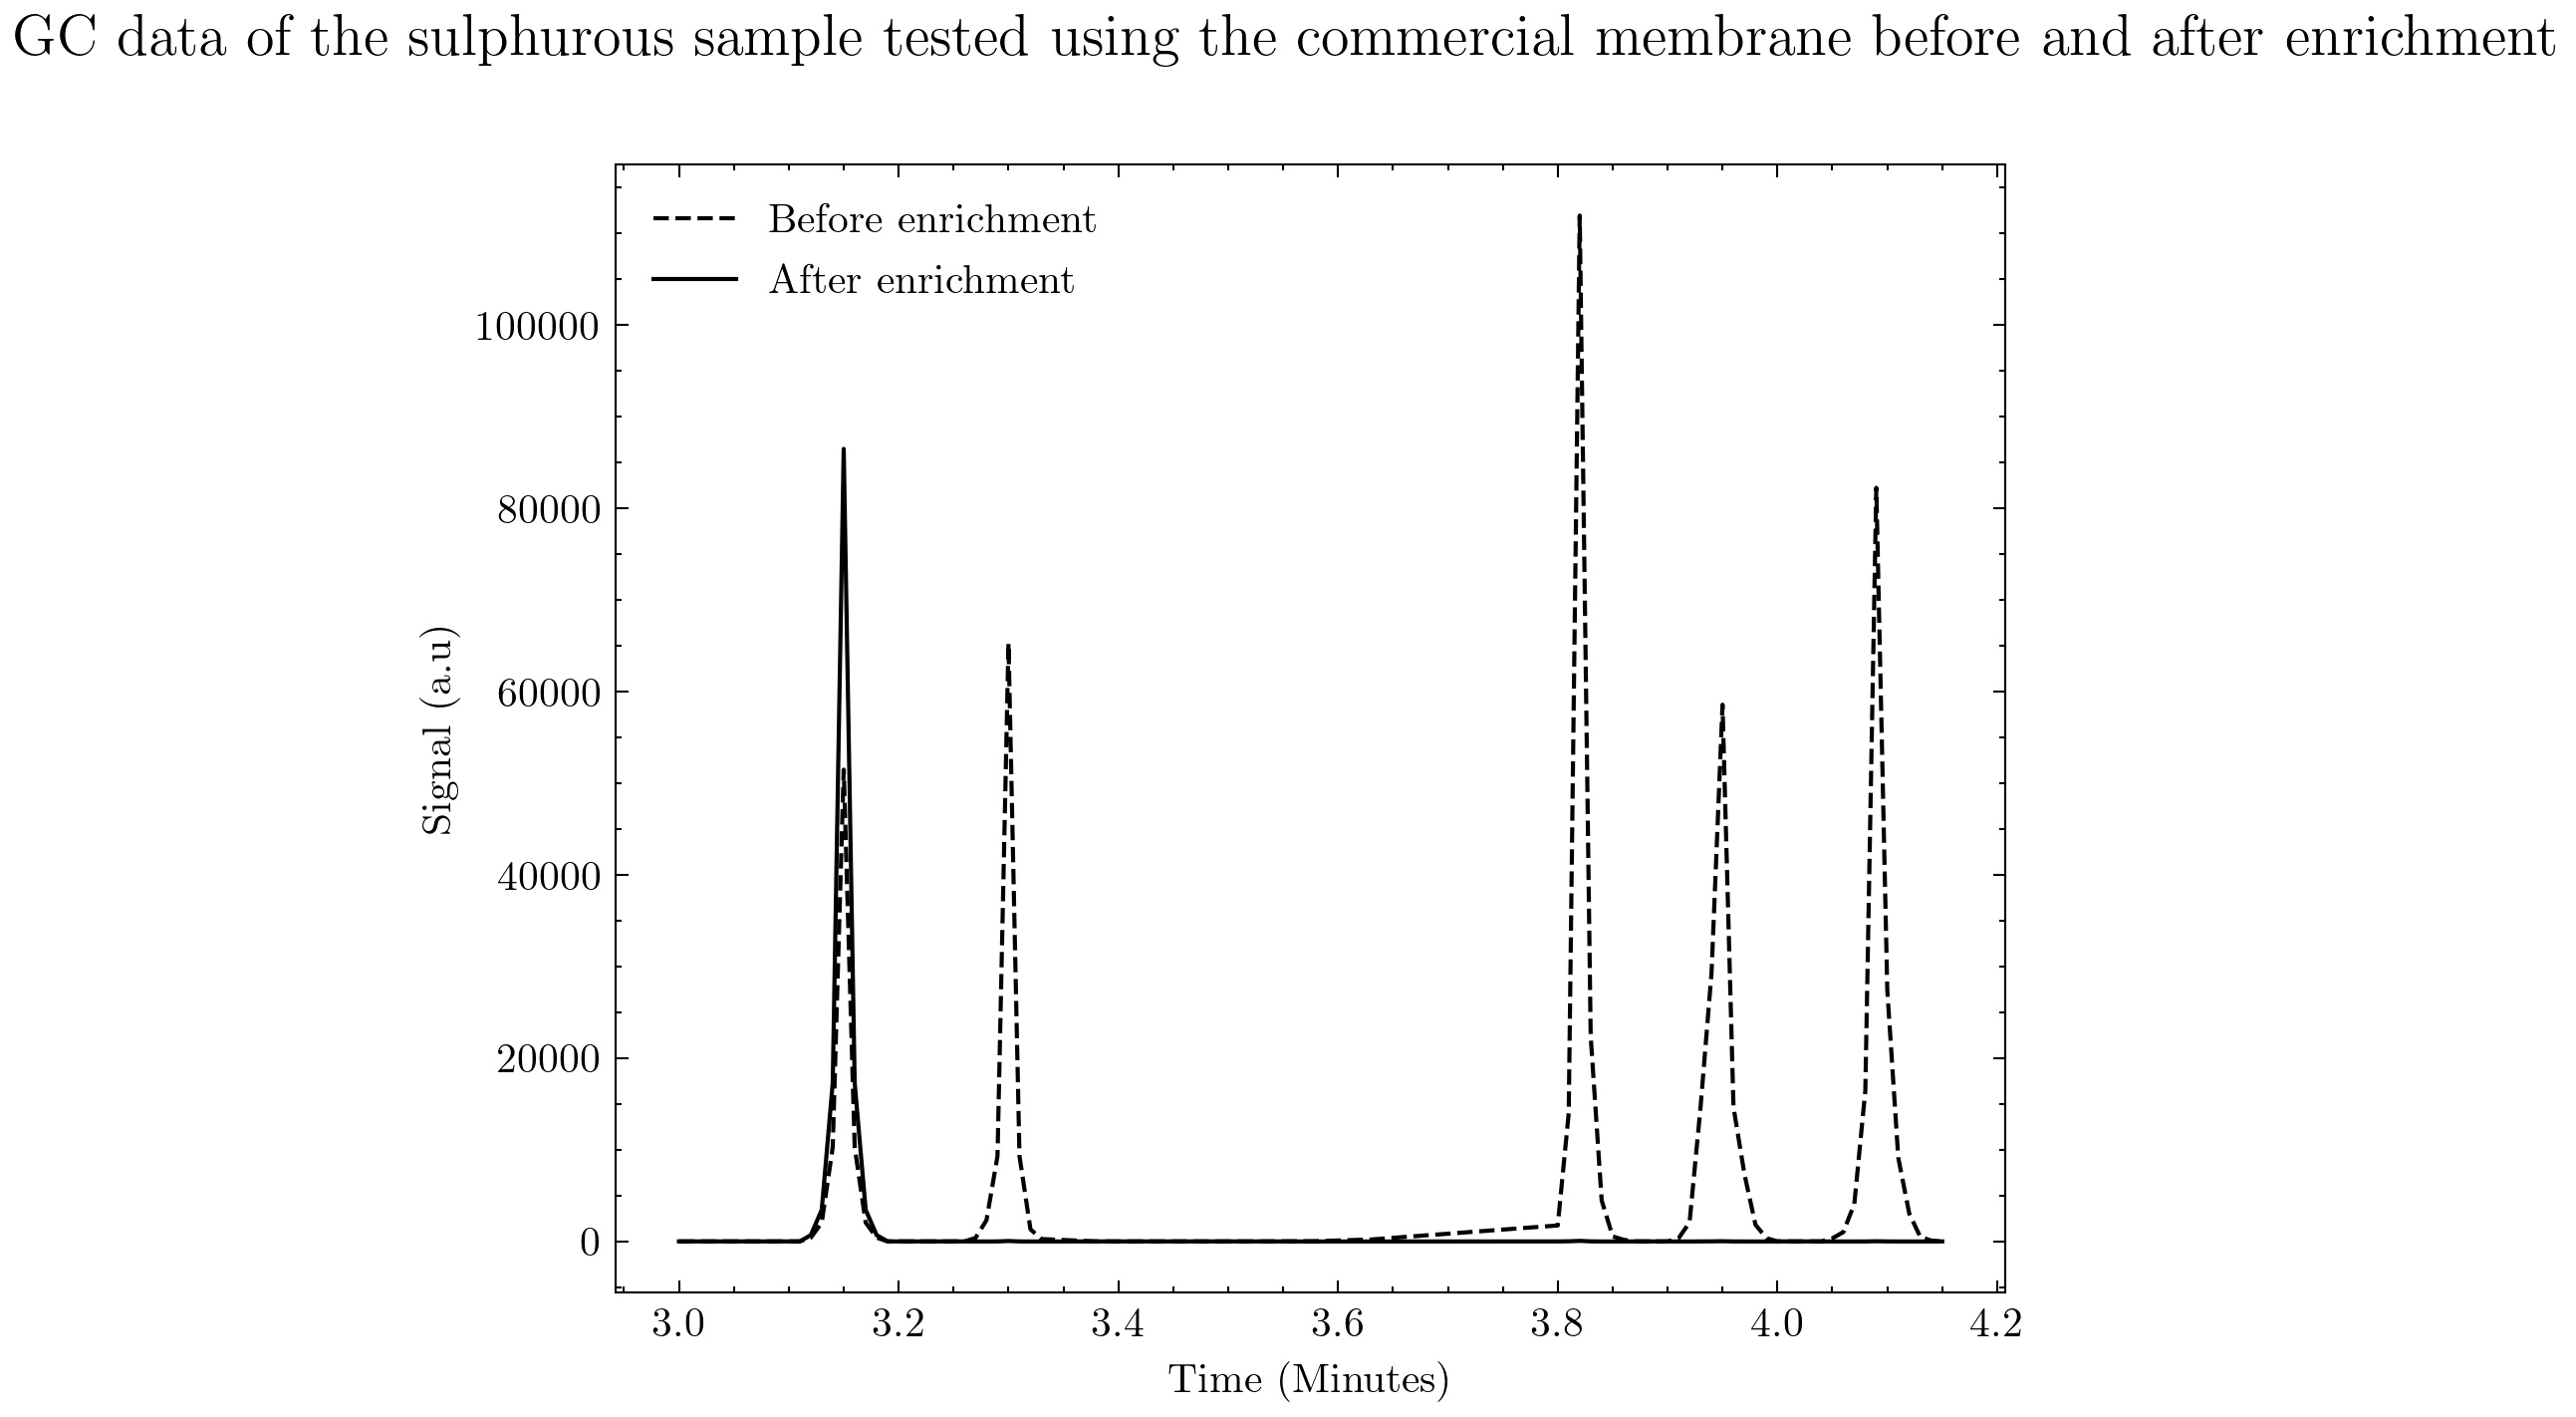
\includegraphics[width=\linewidth, keepaspectratio]{/Users/marc/Thesis/Chapter5/sulfcomgc.jpg}
    \caption{GC-SCD data of the sulphurous sample both before and after enrichment with commercial membrane}
    \label{GCSULFCOMM}
\end{figure}

The PdCuZr membrane was tested twice, with both runs ending in failure due to delamination of the membrane after a number of temperature cycles. On the second attempt the heating ramp was lowered to 1 \textdegree C/min in order to put less thermal strain on the membrane. This resulted in the membrane lasting one extra temperature cycle, however made no lasting difference to the result. The reason for this is likely to be the combined force of the extra pressure in the enrichment vessel durting heating, and the multiple heating cooling cycles used over the course of the experiment causing the mismatch between the thermal expansion coefficient betwen the membrane and support to result in membrane failure. 

Since all enrichment experiments failed for the sulphur sample a comparison of the enrichment factors in sulphur containing atmospheres cannot be performed. 

\begin{landscape}
    \begin{figure}
        \centering
        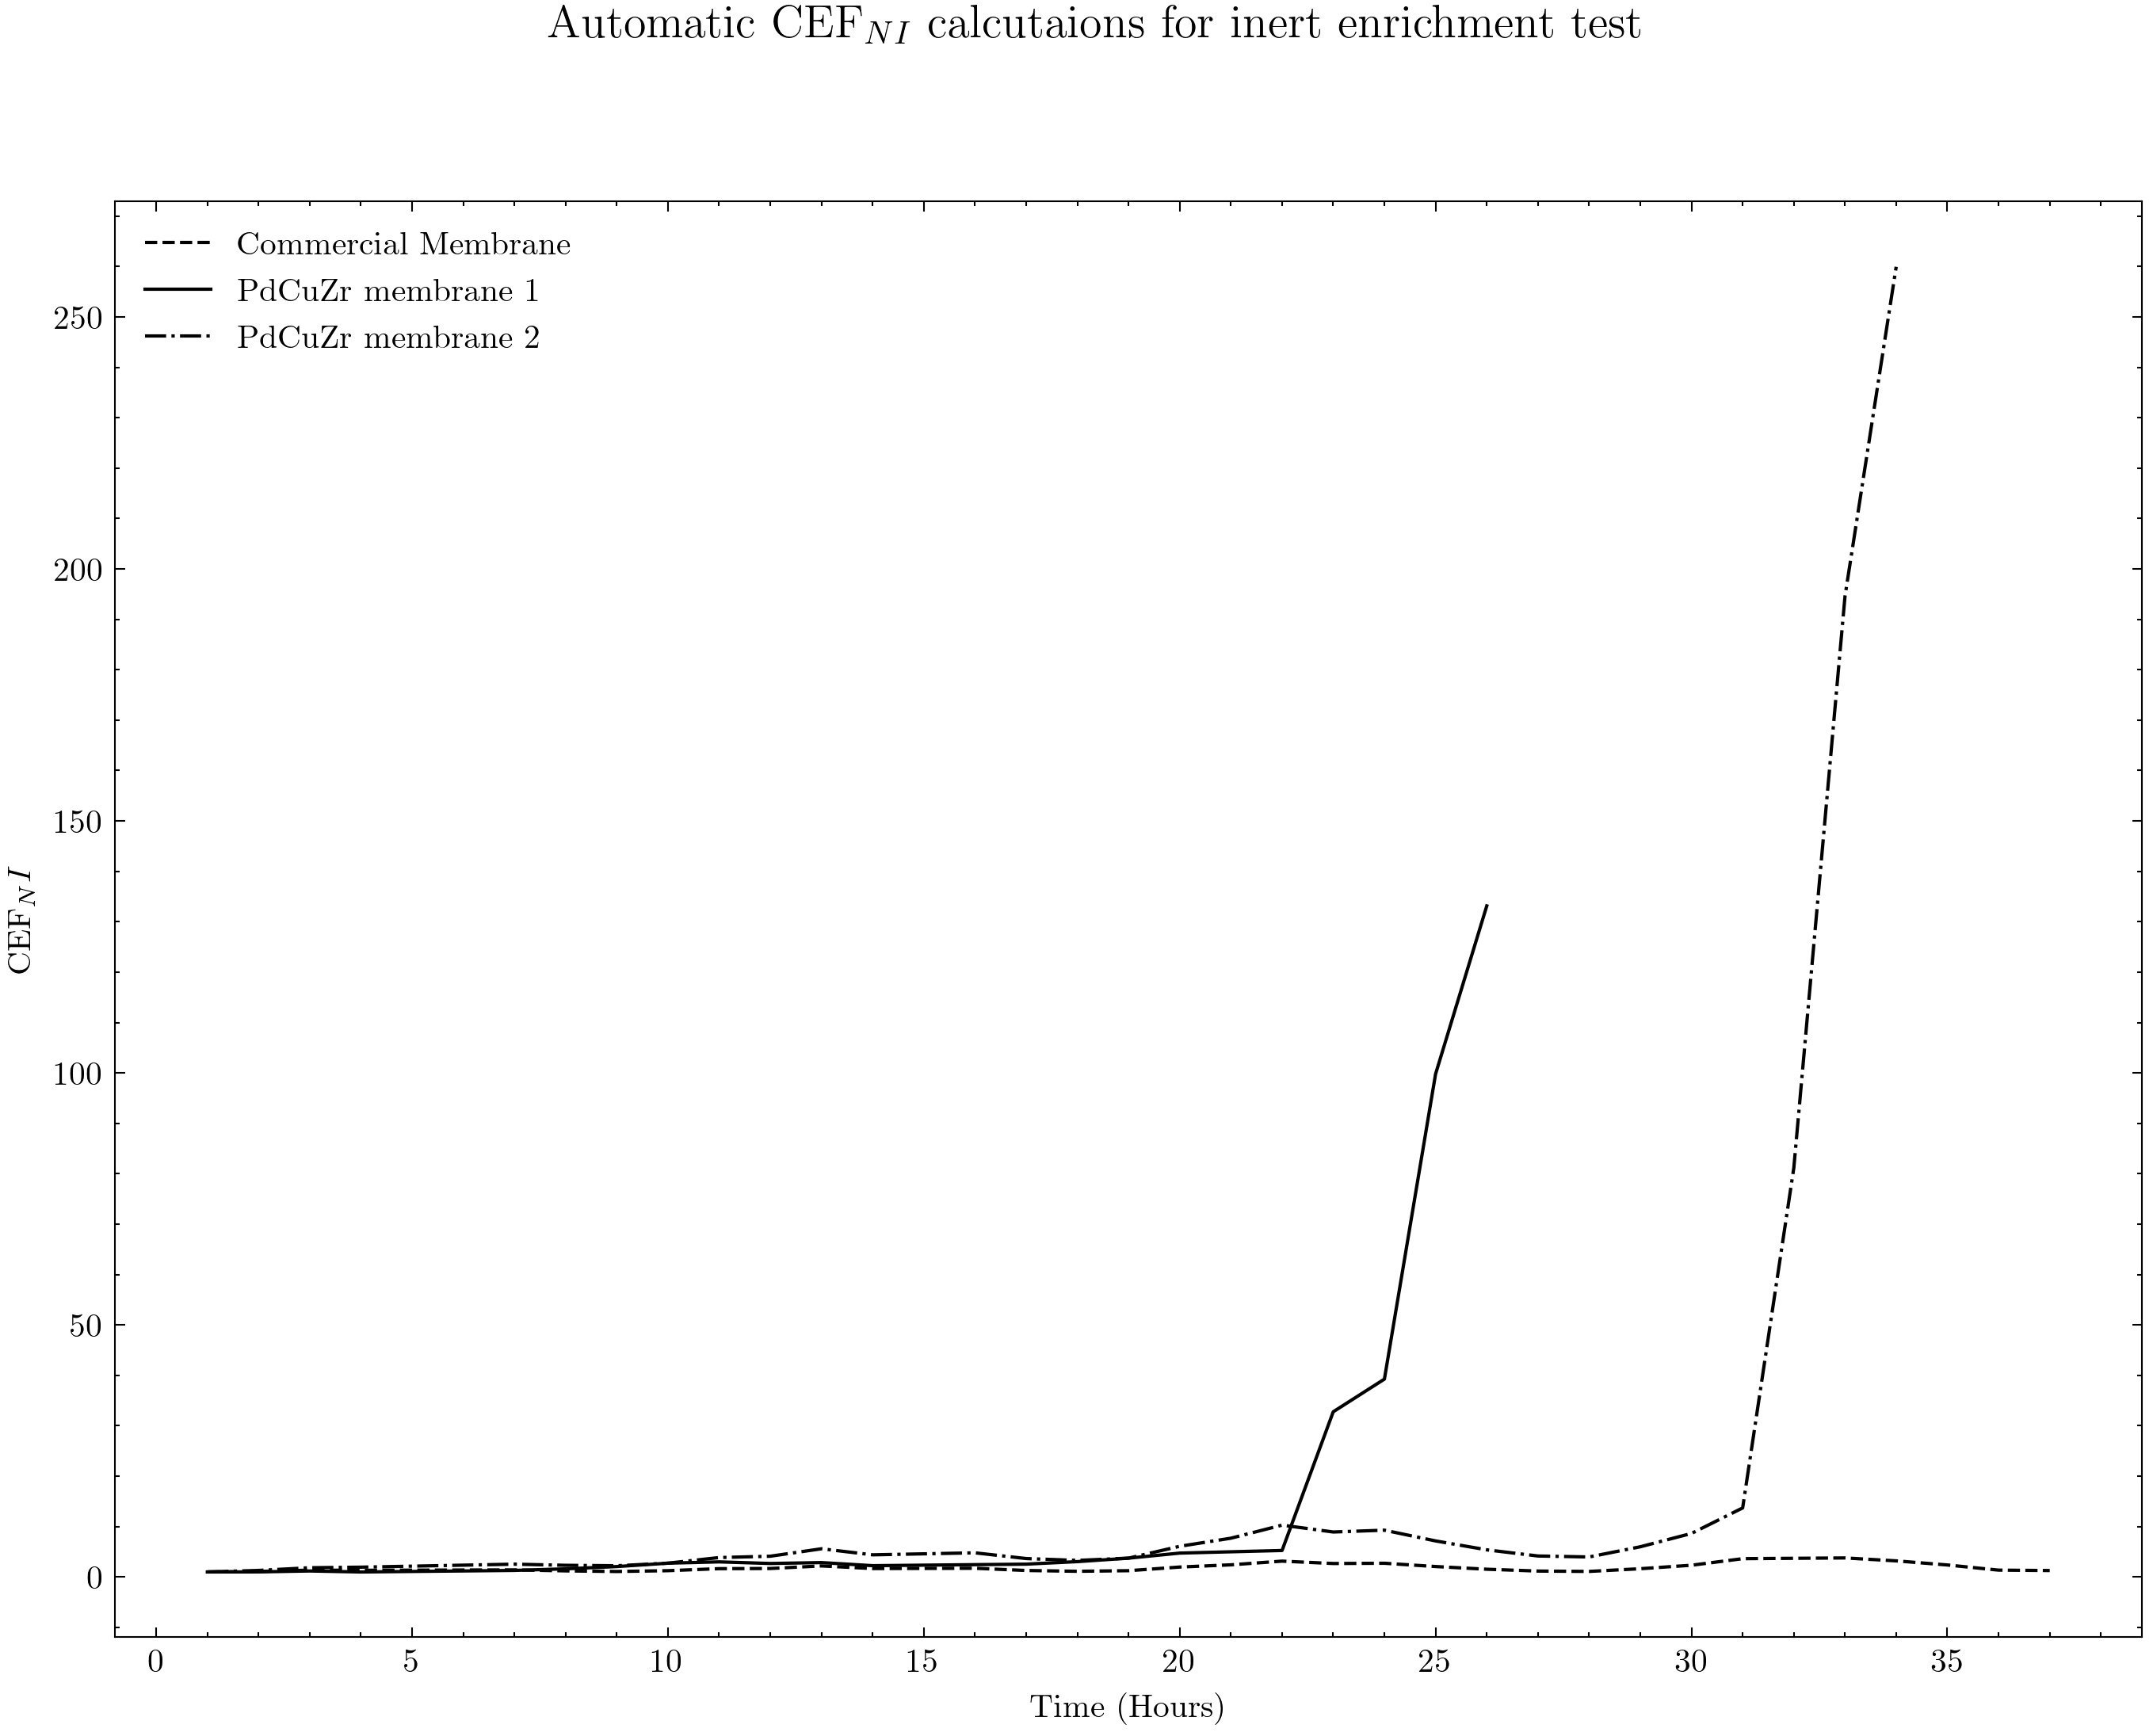
\includegraphics[width=0.9\linewidth, keepaspectratio]{/Users/marc/Thesis/Chapter5/sulfenrichni.jpg}
        \caption{$CEF_{NI}$ over the 40 hour enrichment of the sulphurous hydrogen sample shown in table \ref{exp-sulf}}
        \label{GCSULF}
    \end{figure}
\end{landscape}

\subsection{HRS sample}
The sample taken from the hydrogen refuelling station spiked with krypton as described in \ref{kryptonspike} was enriched using the commercial PdAuAG membrane as this was the only composition able to withstand the conditions required for enrichment. The enrichment was performed over 120 hours. Initial analysis showed that the krypton concentration in the sample before enrichment was 80 \textmu mol/mol and that nitrogen was present in the sample likely due to dead volume within the H\textsubscript{2} qualitizer. The CEF\textsubscript{NI} over the course of the experiment is shown in figure \ref{GCHRS} and predicted that the sample was enriched 55.36 ± 3.4 times using the non-ideal gas law method.

\begin{landscape}
    \begin{figure}
        \centering
        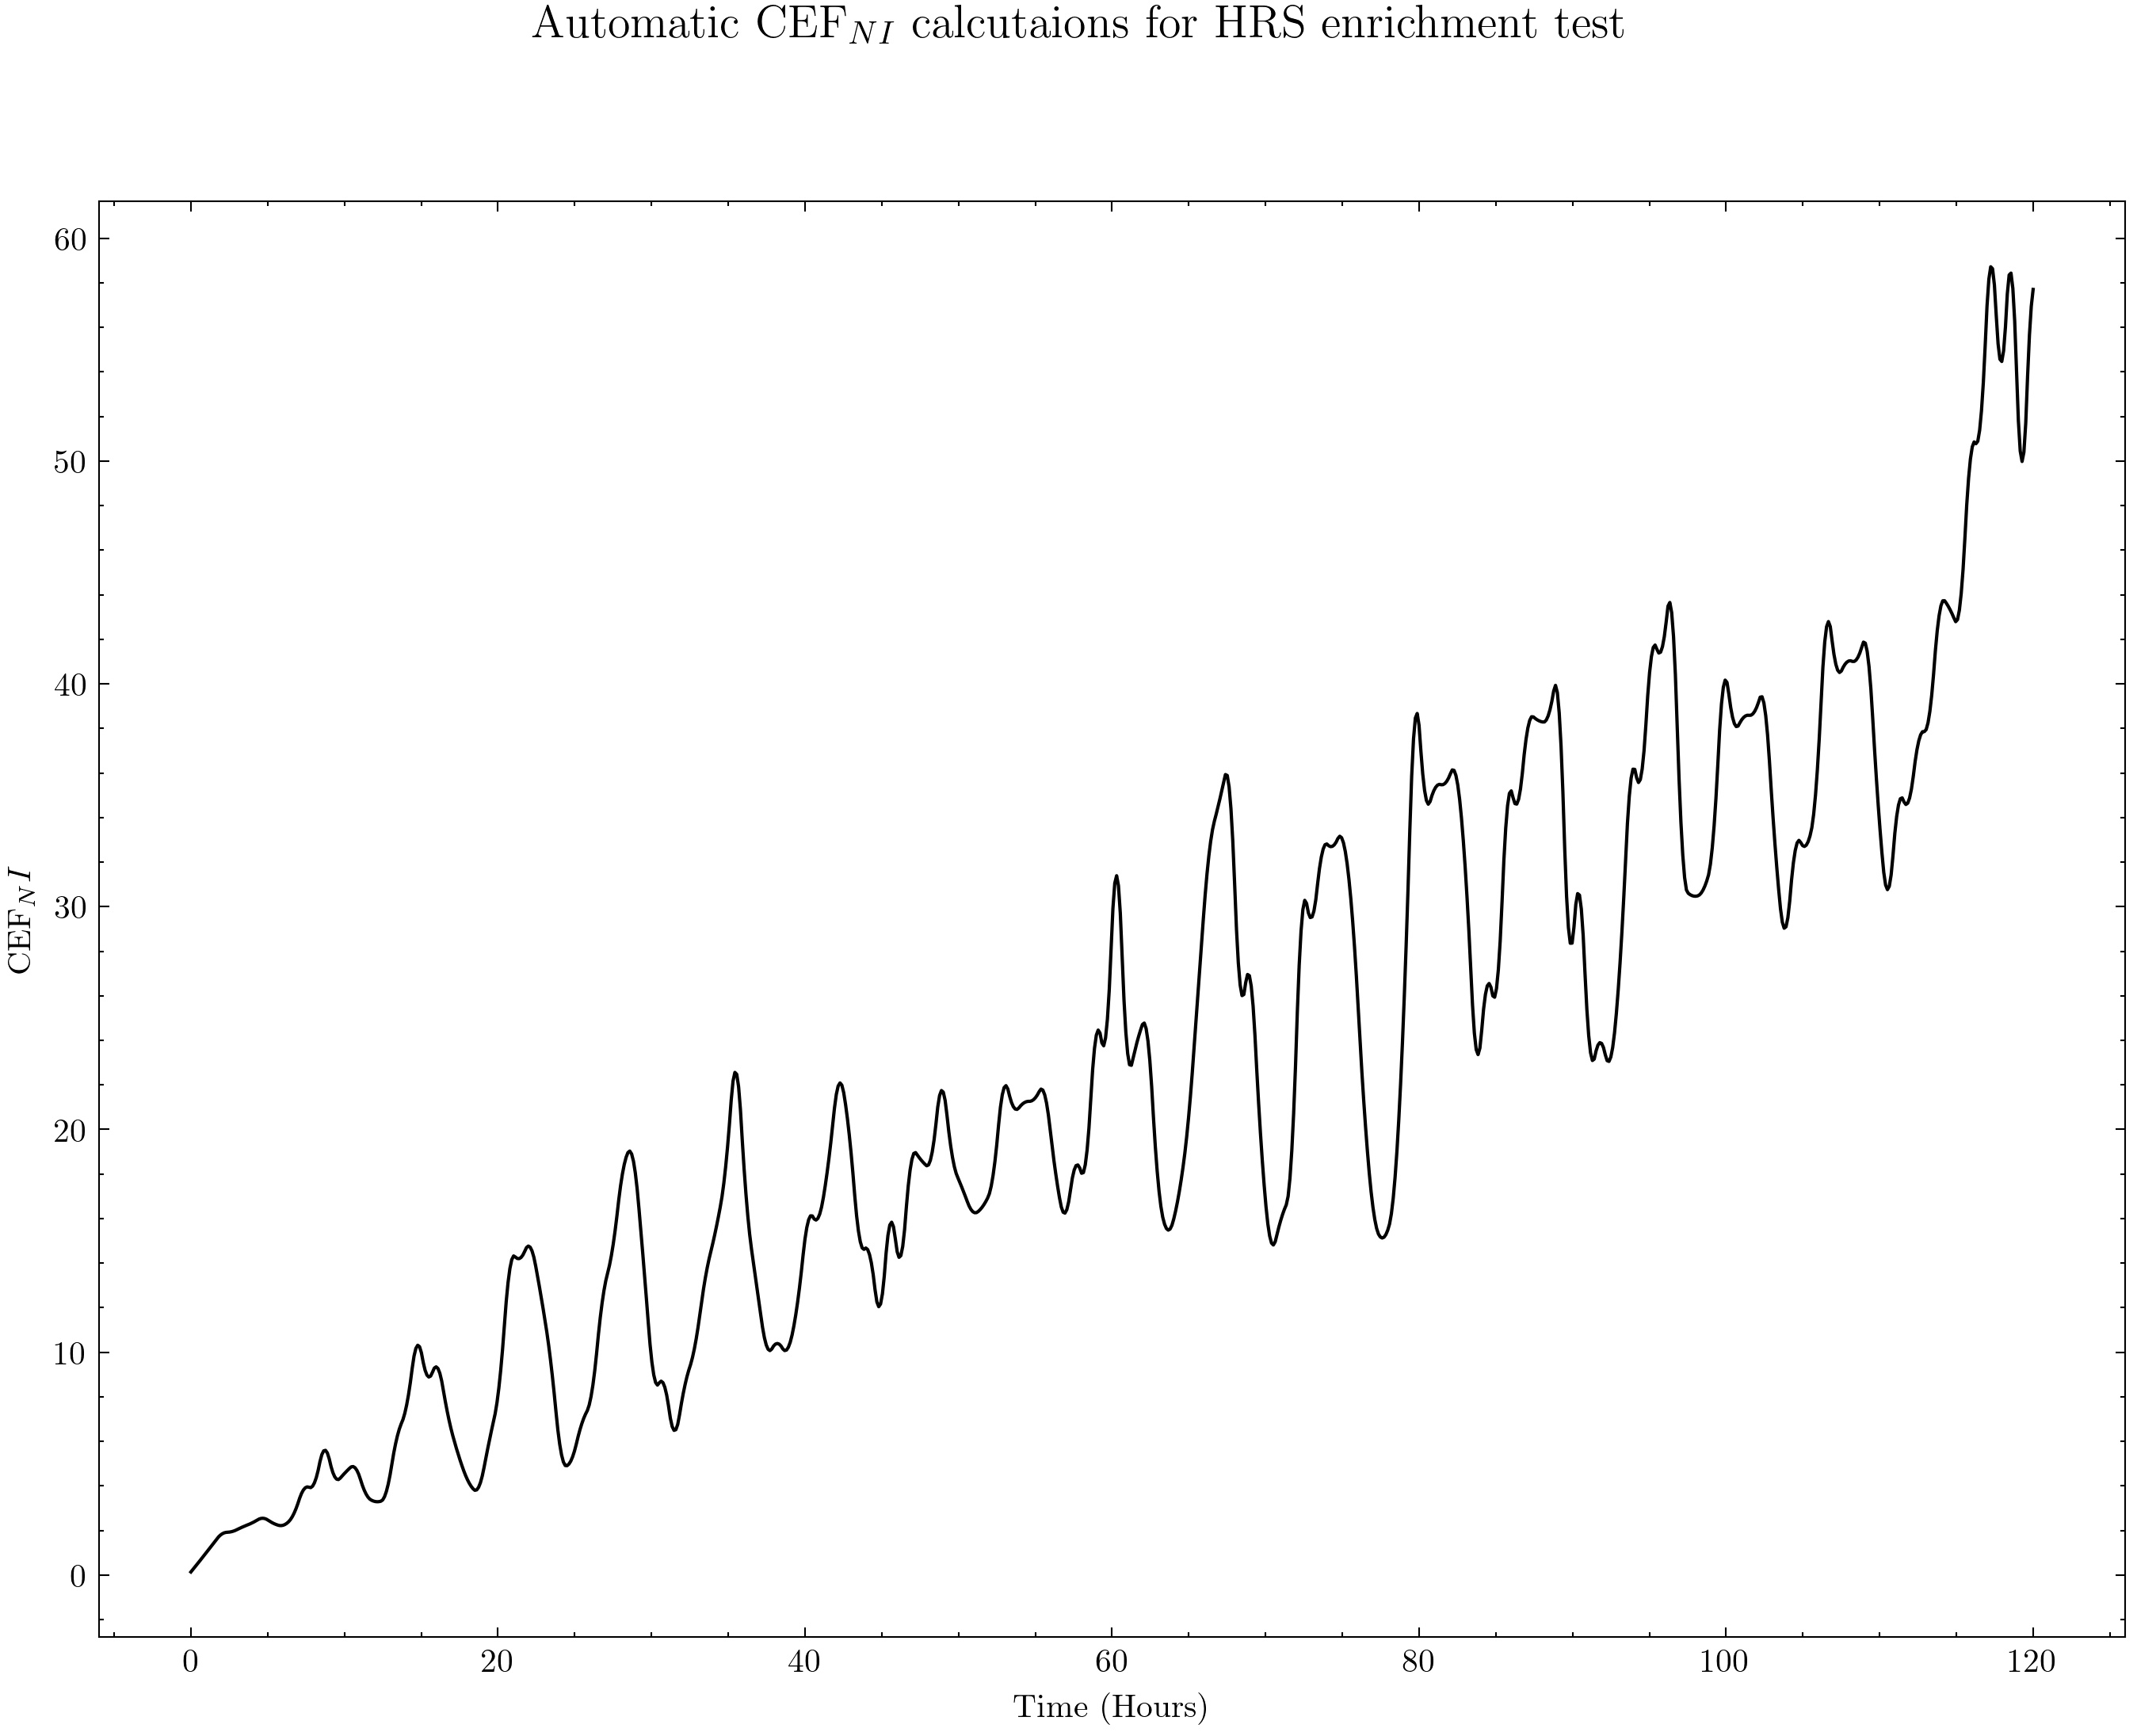
\includegraphics[width=0.9\linewidth, keepaspectratio]{/Users/marc/Thesis/Chapter5/hrsenrichni.jpg}
        \caption{$CEF_{NI}$ over the 120 hour enrichment of the HRS hydrogen sample}
        \label{GCHRS}
    \end{figure}
\end{landscape}

The sample was enriched to an enrichment factor of 41.76 ± 2.3 as shown by the increase of krypton and nitrogen concentrations shown in figure xx. These peaks corresponded to concentrations of 3374 ± 32 \textmu mol/mol of krypton and 957 ± 10.6 \textmu mol/mol of Nitrogen respectivley. Using the tracer enrichment factor this corresponds to an initial concentration  of 22.91 ± 3.2  \textmu mol/mol of Nitrogen  in the hydrogen sample. The results in the enriched sample also show a new peak at 2.4 minutes which corresponds to Argon, thereby proving that the method can be used to quantify impurities which were below the limit of detection of the detector in the initial sample. Due to the small size of the peak, quantifying the concentration was difficult and a higher enrichment factor would be required to accurately determine this. Unfortunately due to interrruptions from COVID-19 adequate time was not avaliable to perform this test. 

\begin{figure}[H]
    \centering
    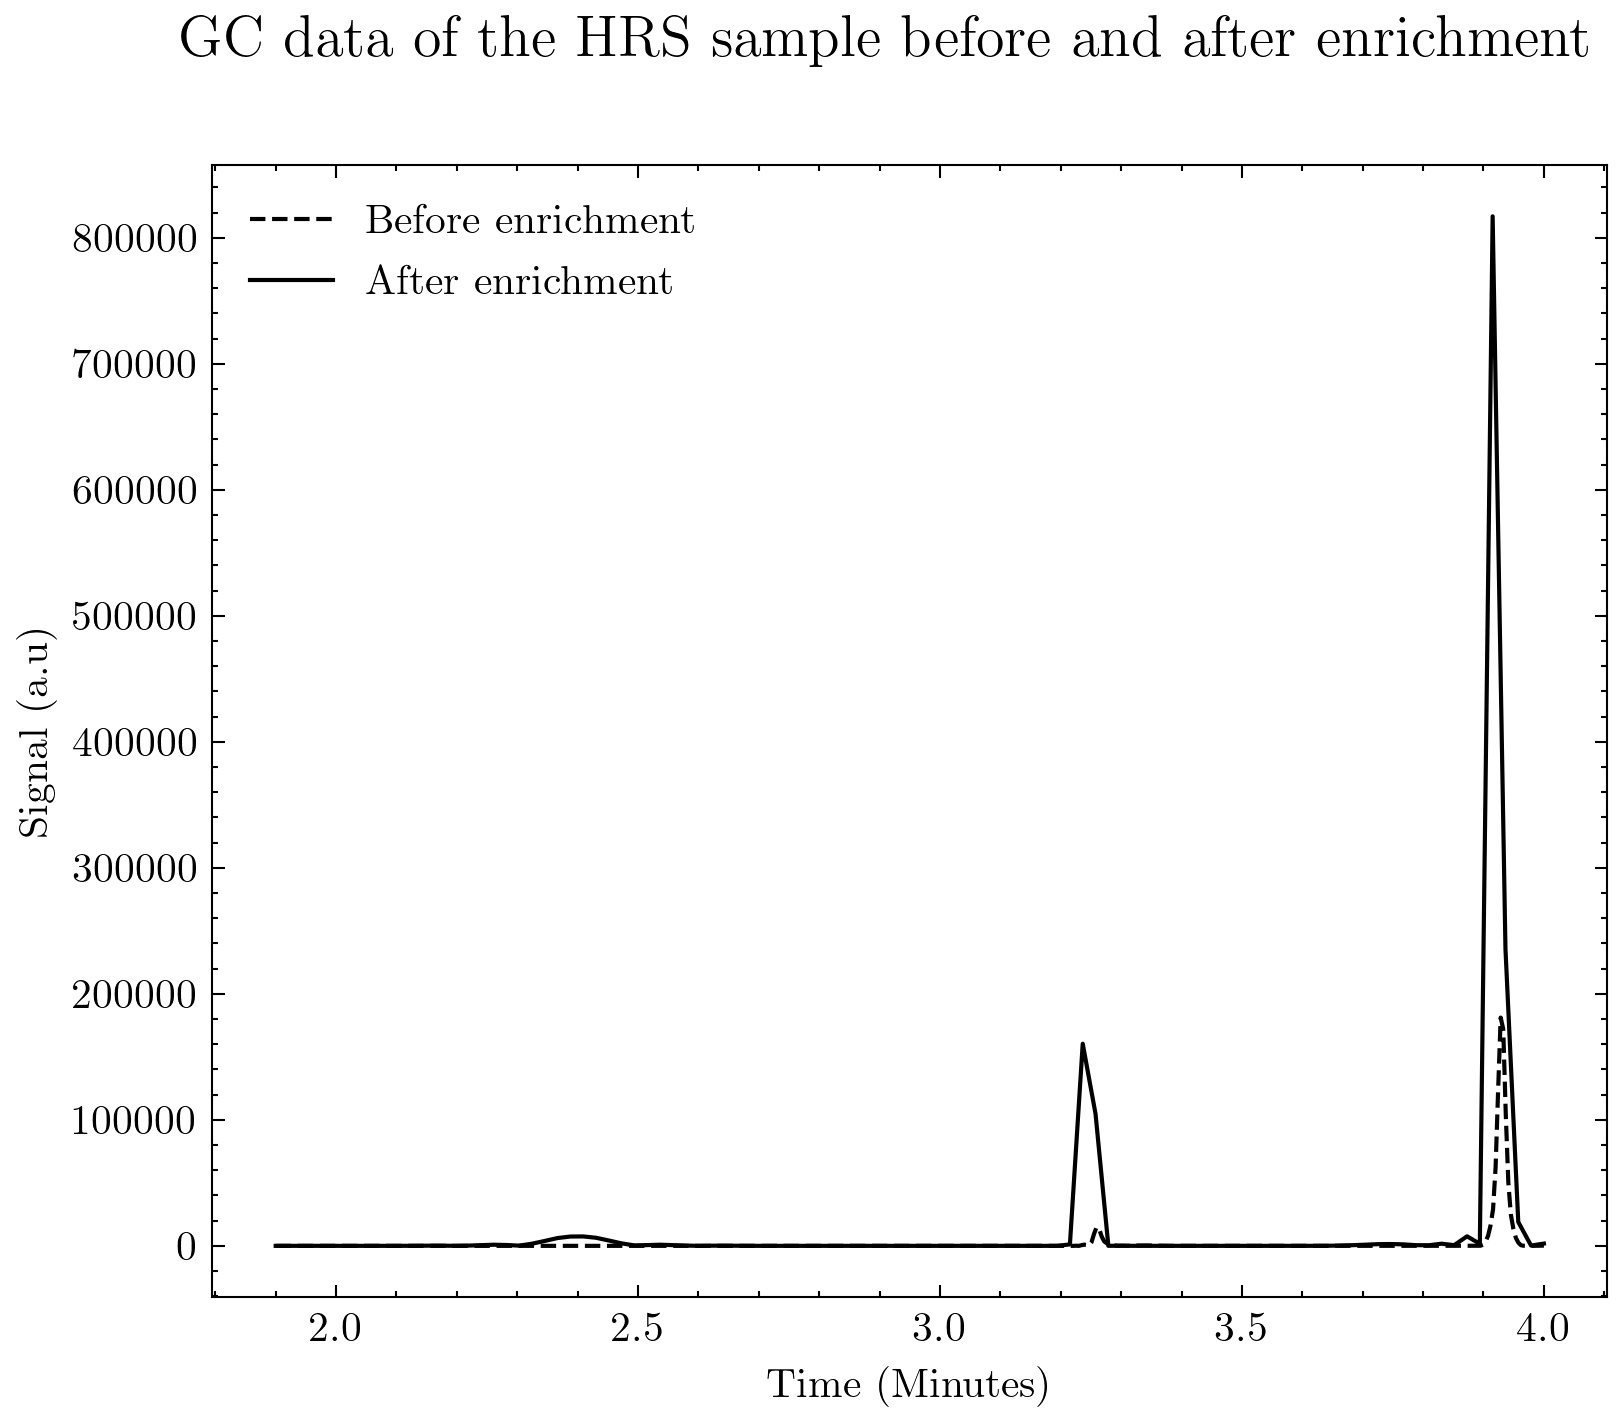
\includegraphics[width=\linewidth, keepaspectratio]{/Users/marc/Thesis/Chapter5/hrsgc.jpg}
    \caption{GC-PDHID data of the HRS sample both before and after enrichment with commercial membrane}
    \label{HRSGCENRICH}
\end{figure}

\section{Conclusion}
The new enrichment device was tested using 3 hydrogen samples, a sample containing only inert impurities in order to test the device functions as required, a sulphur containing sample to test how the PdCuZr membrane identified as the best membrane in chapter \label{proc-testingchapref}, and a sample taken from a hydrogen refuelling station. The inert sample was successsfully enriched to 50x and using the tracer enrichment method using krypton the initial concentration of nitrogen was calculated to within 2\% of it's original value. 

The sulphur tests resulted in failure of all membranes used. For the commercial membrane this was due to high reactivity with the sulphur compounds which was also identified in chapter 5. For the PdCuZr membrane this was due to material instability and further work is required to manufacture the ceramic supported membrane to be able to withstand temperature cycling. 

For the first time enrichment was performed on a real sample from a hydrogen refuelling station, proving both that the method is viable for analysis of real world hydrogen samples, and the protocol for spiking a hydrogen sample with krypton gas is approptiate. The sample was enriched 41 times and was able to accurately determine that the concentration of nitrogen in the sample before enrichment was 22.91 \textmu mol/mol. Enrichment also revealed the presence of Argon in the sample, which would not have been present in the analysis otherwise, further proving that the technique can provide a more accurate composition analysis of fuel grade hydrogen, past what is possible with commercial analysers.

\bibliographystyle{unsrtnat}
\bibliography{library.bib}